\begin{figure}[H]
    \centering
    \begin{minipage}{0.33\textwidth}
        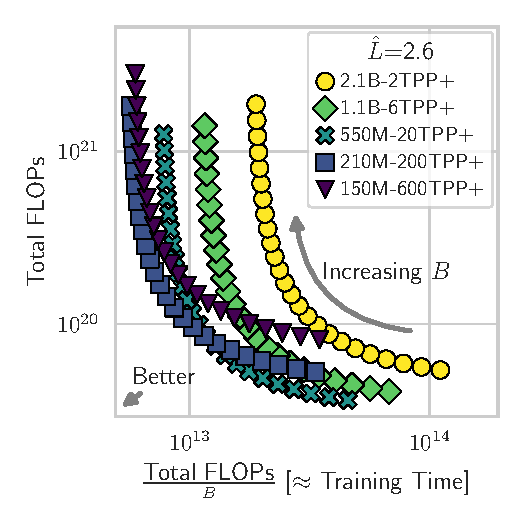
\includegraphics[trim={0.3cm 0.4cm 0.3cm 0.3cm}, clip, width=\linewidth]{pdffigs/pareto.l=2.6.v3.pdf}
    \end{minipage}\hfill
    \begin{minipage}{0.33\textwidth}
        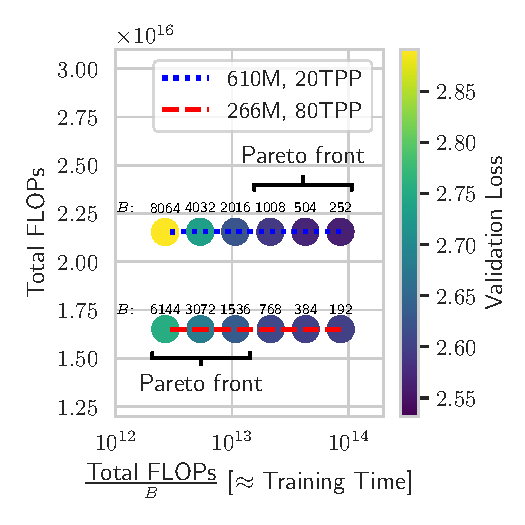
\includegraphics[trim={0.3cm 0.4cm 0.3cm 0.3cm}, clip, width=\linewidth]{pdffigs/loss_data.241005_batchsizes.flop_flops3.pdf}
    \end{minipage}\hfill
    \begin{minipage}{0.33\textwidth}
        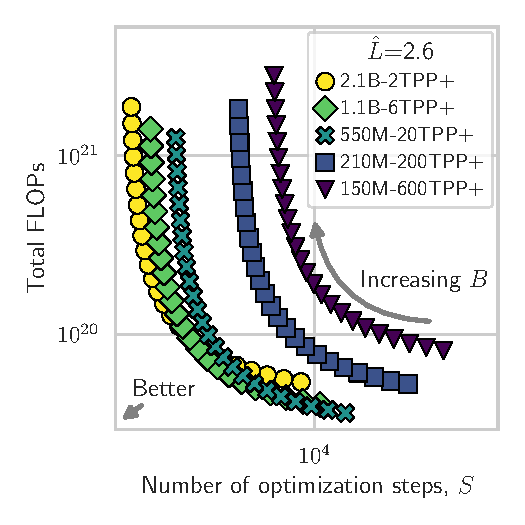
\includegraphics[trim={0.3cm 0.4cm 0.3cm 0.3cm}, clip, width=\linewidth]{pdffigs/pareto.l=2.6.v3.STEPS_ONLY.pdf}
    \end{minipage}
    \caption{($\leftfig$): Iso-loss curves illustrating time--compute
      Pareto frontier ($\lhat$=2.6). As $B$ increases along curves,
      more compute (y-axis), but less time (x-axis) is required. Here
      time $\propto \nicefrac{\totflopstext}{B}$.  ($\middlefig$):
      Observed runs where some overtrained models (red line) are on
      frontier: $L$ in color, $B$ labeled.  ($\rightfig$): Iso-loss
      curves, but where time = steps; a very different frontier
      emerges.\label{fig:paretos}}
\end{figure}
